% Appendix C

\chapter{Experiment Walkthrough}
\label{an:walkthrough}

%----------------------------------------------------------------------------------------

\noindent The following are screenshots of each page of the experiment website. First, participants were greeted and given an overview of the experiment procedure (\autoref{fig:web_main}). Next, participants were asked to complete the initial questionnaire (\autoref{fig:web_initial}). After submitting it, they were presented with the translation brief for the three translation tasks on a page on its own (\autoref{fig:web_brief}). The aim was for participants to read it and pay attention to it before starting the translations. Participants were told that the brief would be available on the following pages should they need to read it again.

\begin{figure}[h]
\myfloatalign
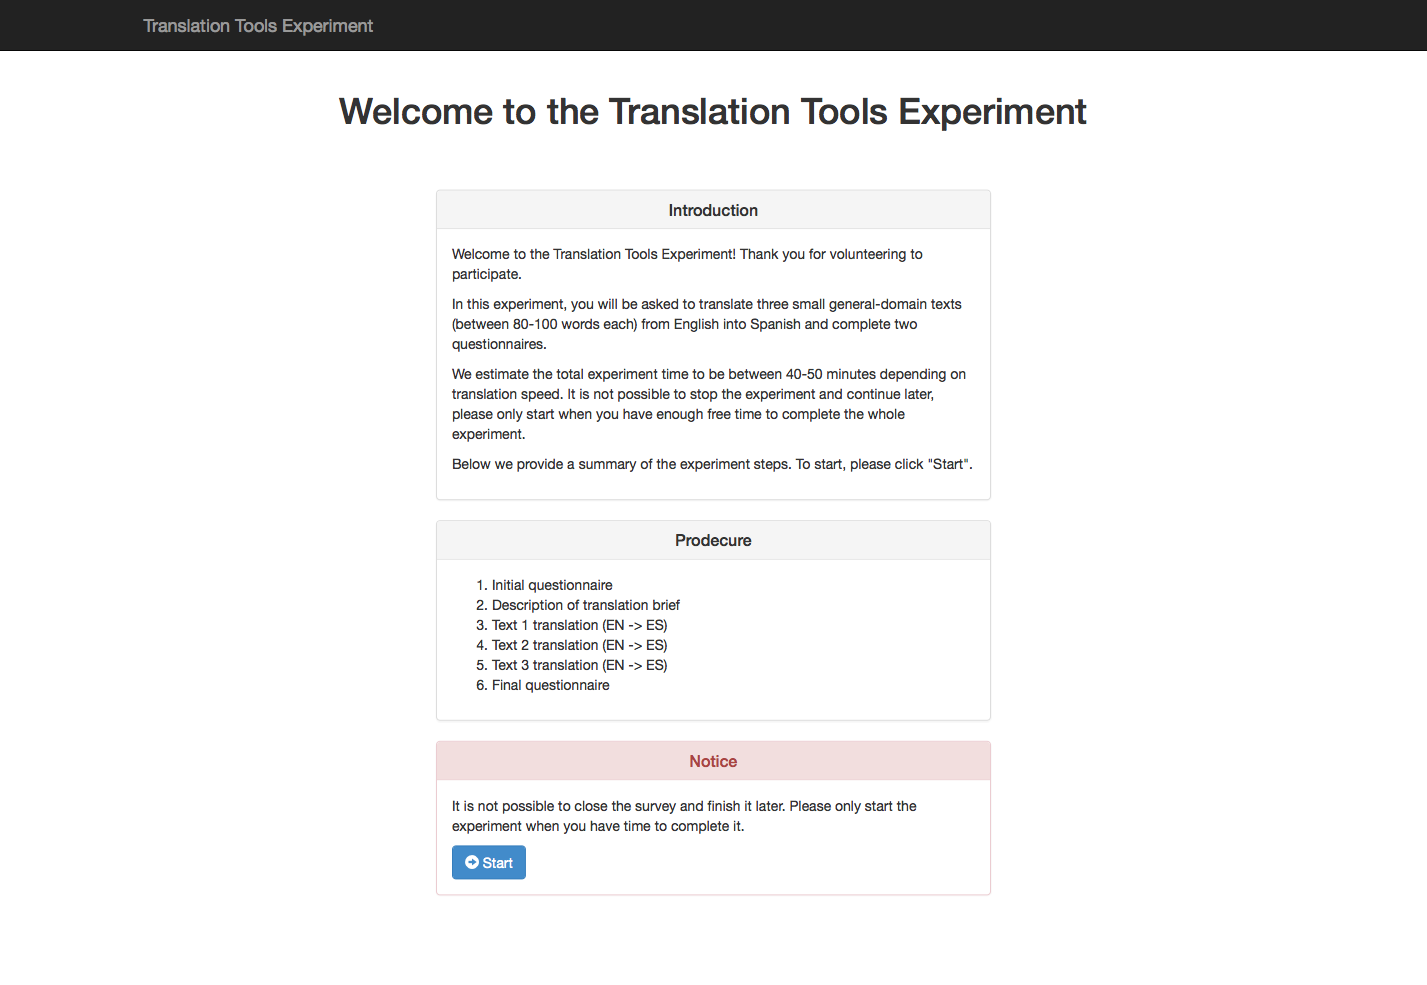
\includegraphics[width=\textwidth]{img/web/web_1.png}
\caption{Website (Page 1). Main page with a general overview of the experiment.}
\label{fig:web_main}
\end{figure}

\begin{figure}[h]
\myfloatalign
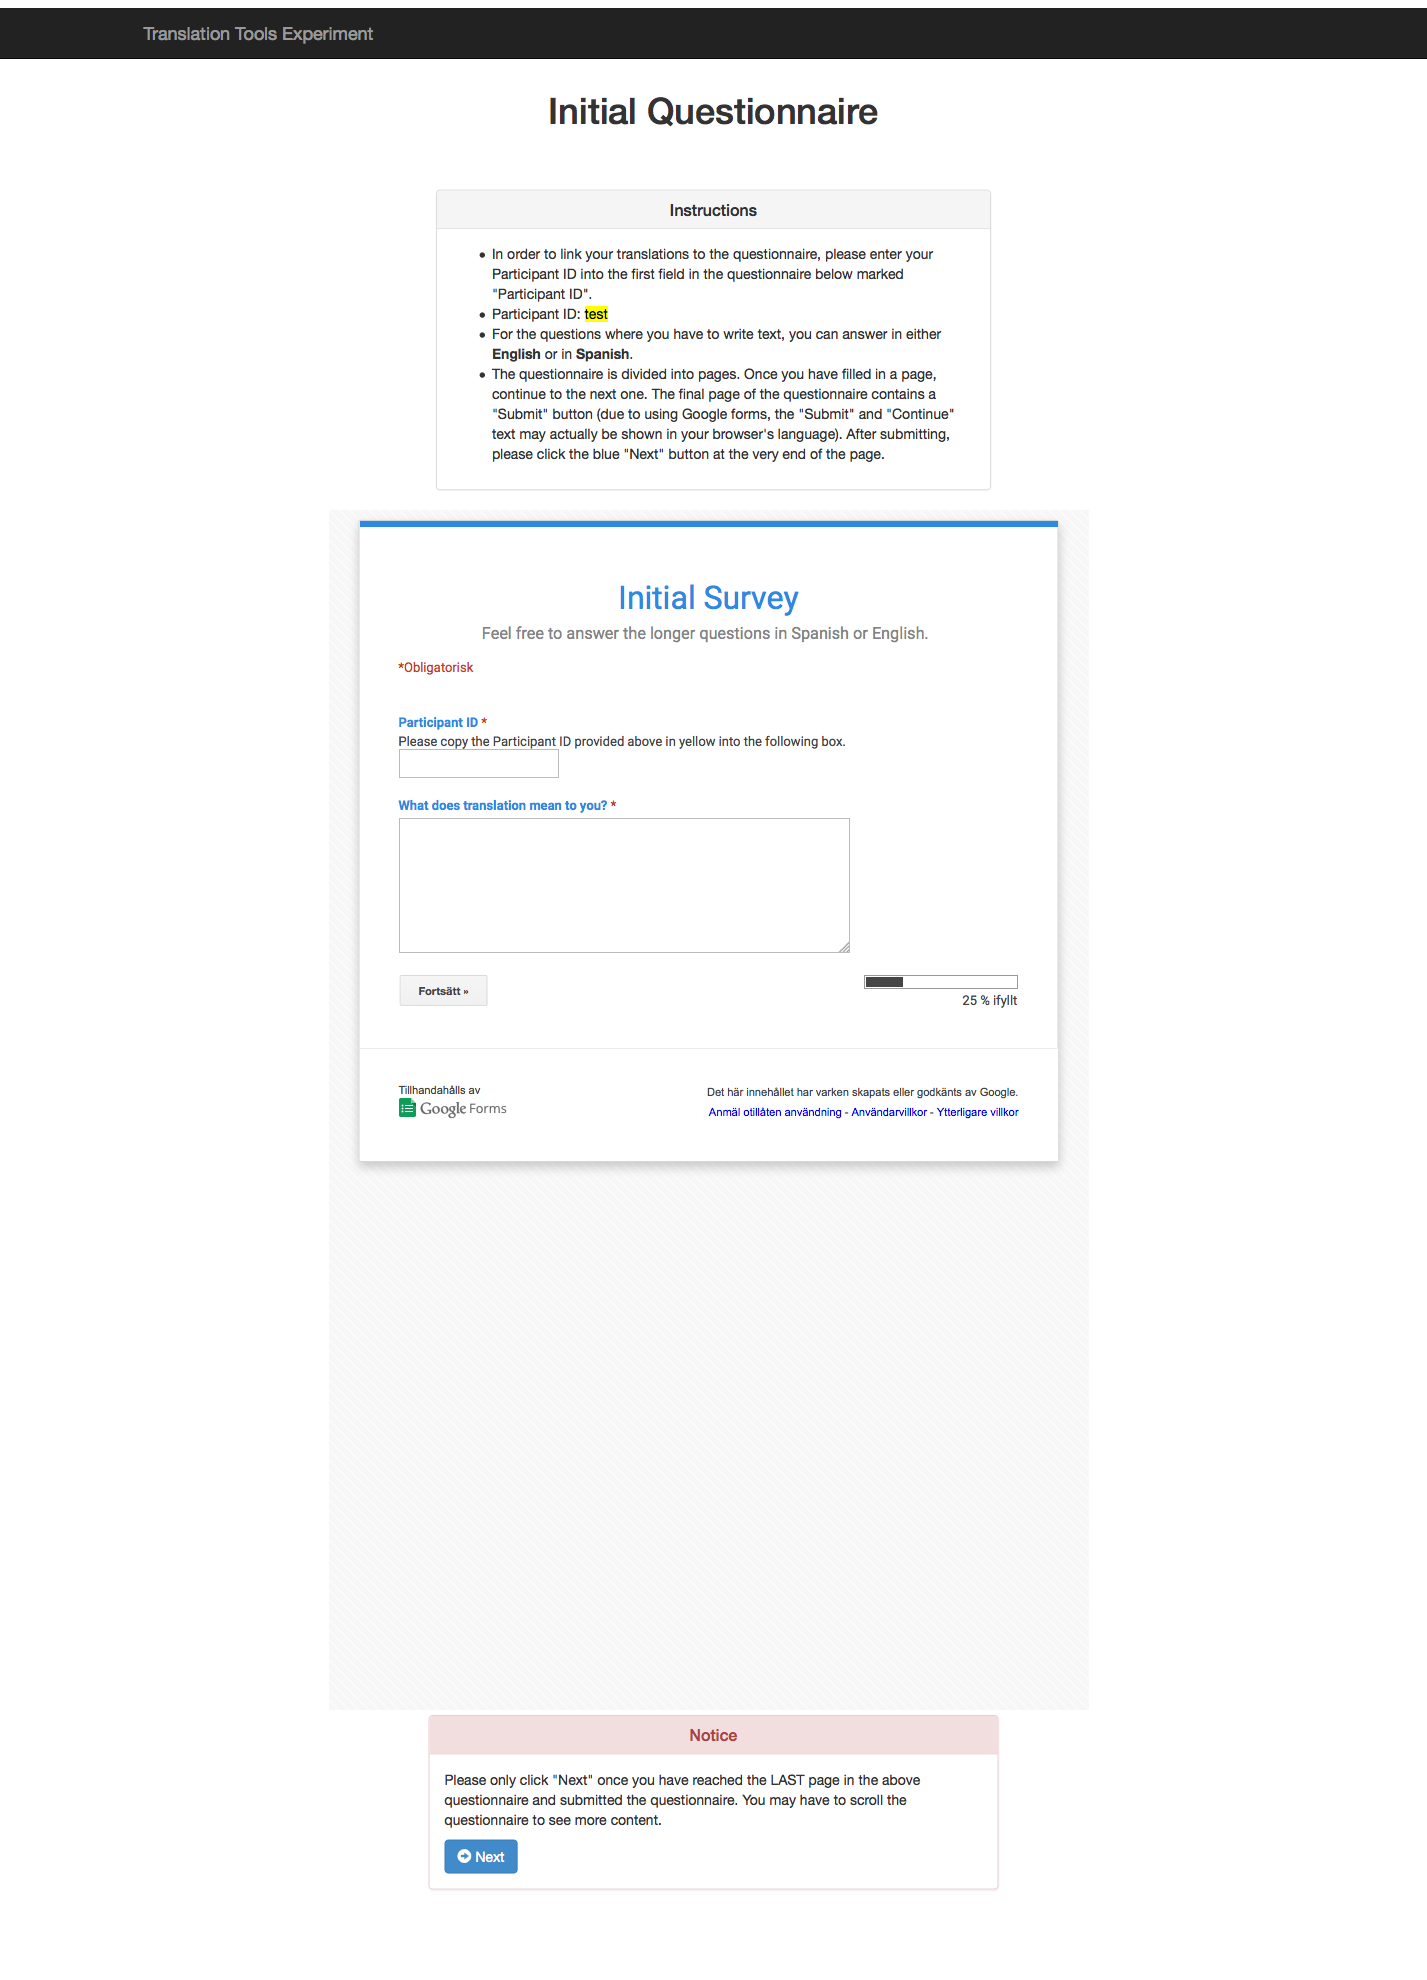
\includegraphics[width=\textwidth]{img/web/web_2.png}
\caption{Website (Page 2). Participants answer the initial questionnaire.}
\label{fig:web_initial}
\end{figure}

\begin{figure}[h]
\myfloatalign
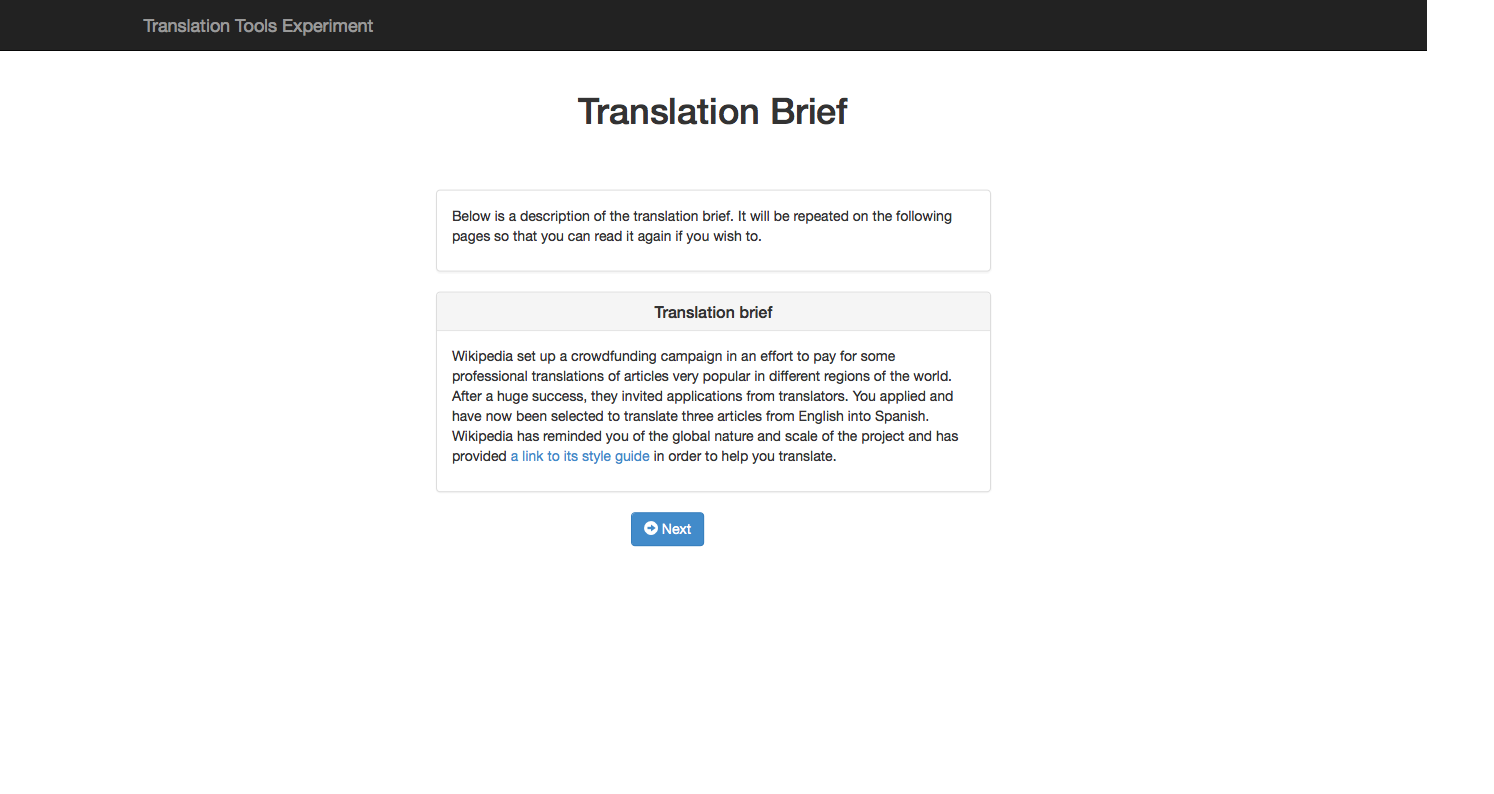
\includegraphics[width=\textwidth]{img/web/web_3.png}
\caption{Website (Page 3). Translation brief description.}
\label{fig:web_brief}
\end{figure}

Then, participants had to carry out the three translations. At the top of each page, instructions were provided for each setup and the translation brief was included. First, the \scratch setup (\autoref{fig:web_scratch}). Second, the \ac{PE} setup (\autoref{fig:web_pe}). Third, the \style setup (\autoref{fig:web_style}). The texts were presented according to the order participants had been provided in the initial link.

\begin{figure}[h]
\myfloatalign
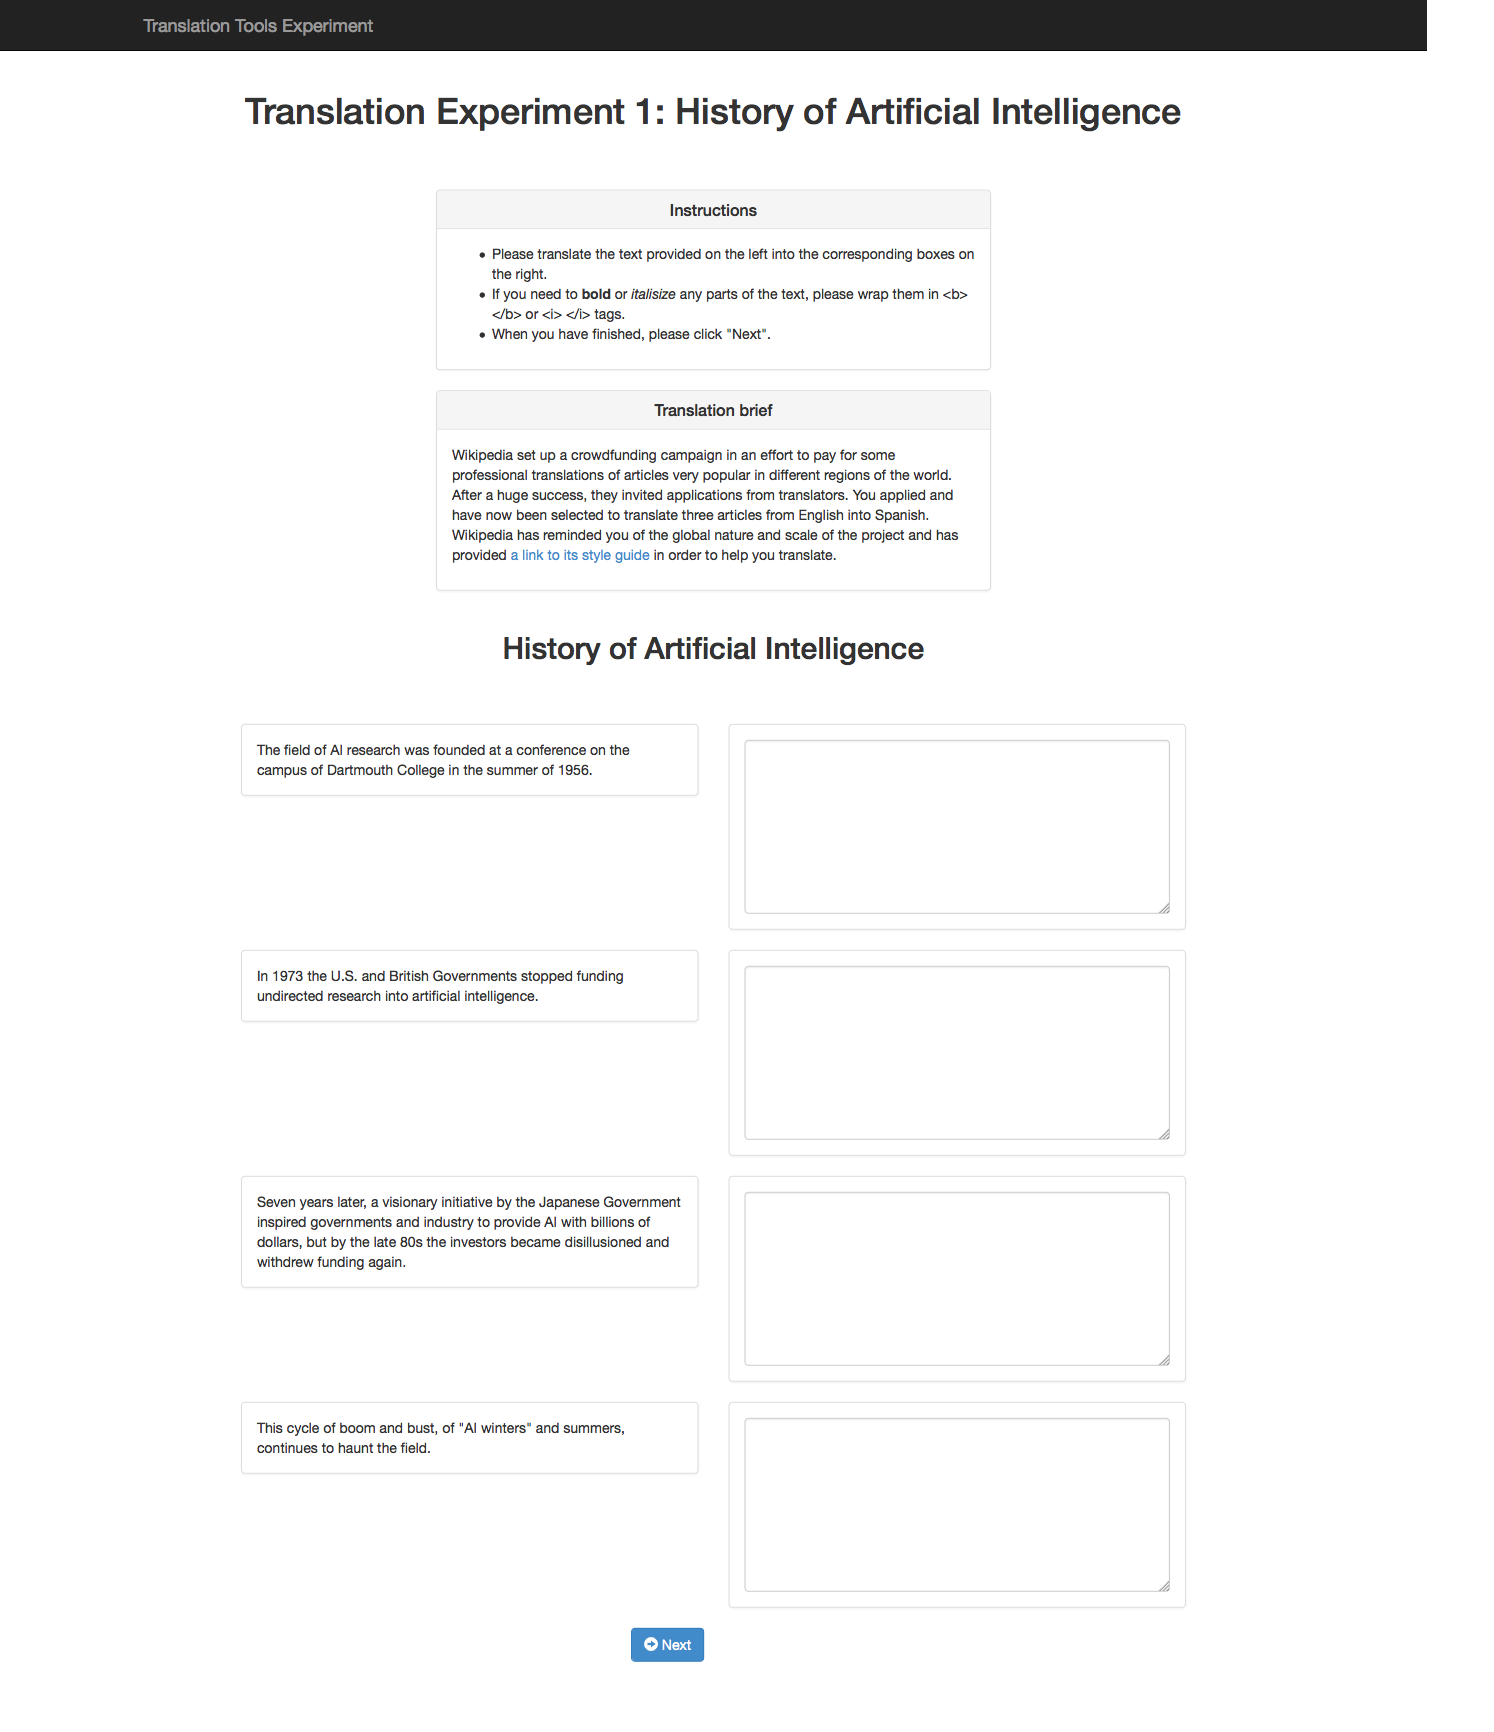
\includegraphics[width=\textwidth]{img/web/web_4.png}
\caption{Website (Page 4). Participants translate in the from-scratch setup.}
\label{fig:web_scratch}
\end{figure}

\begin{figure}[h]
\myfloatalign
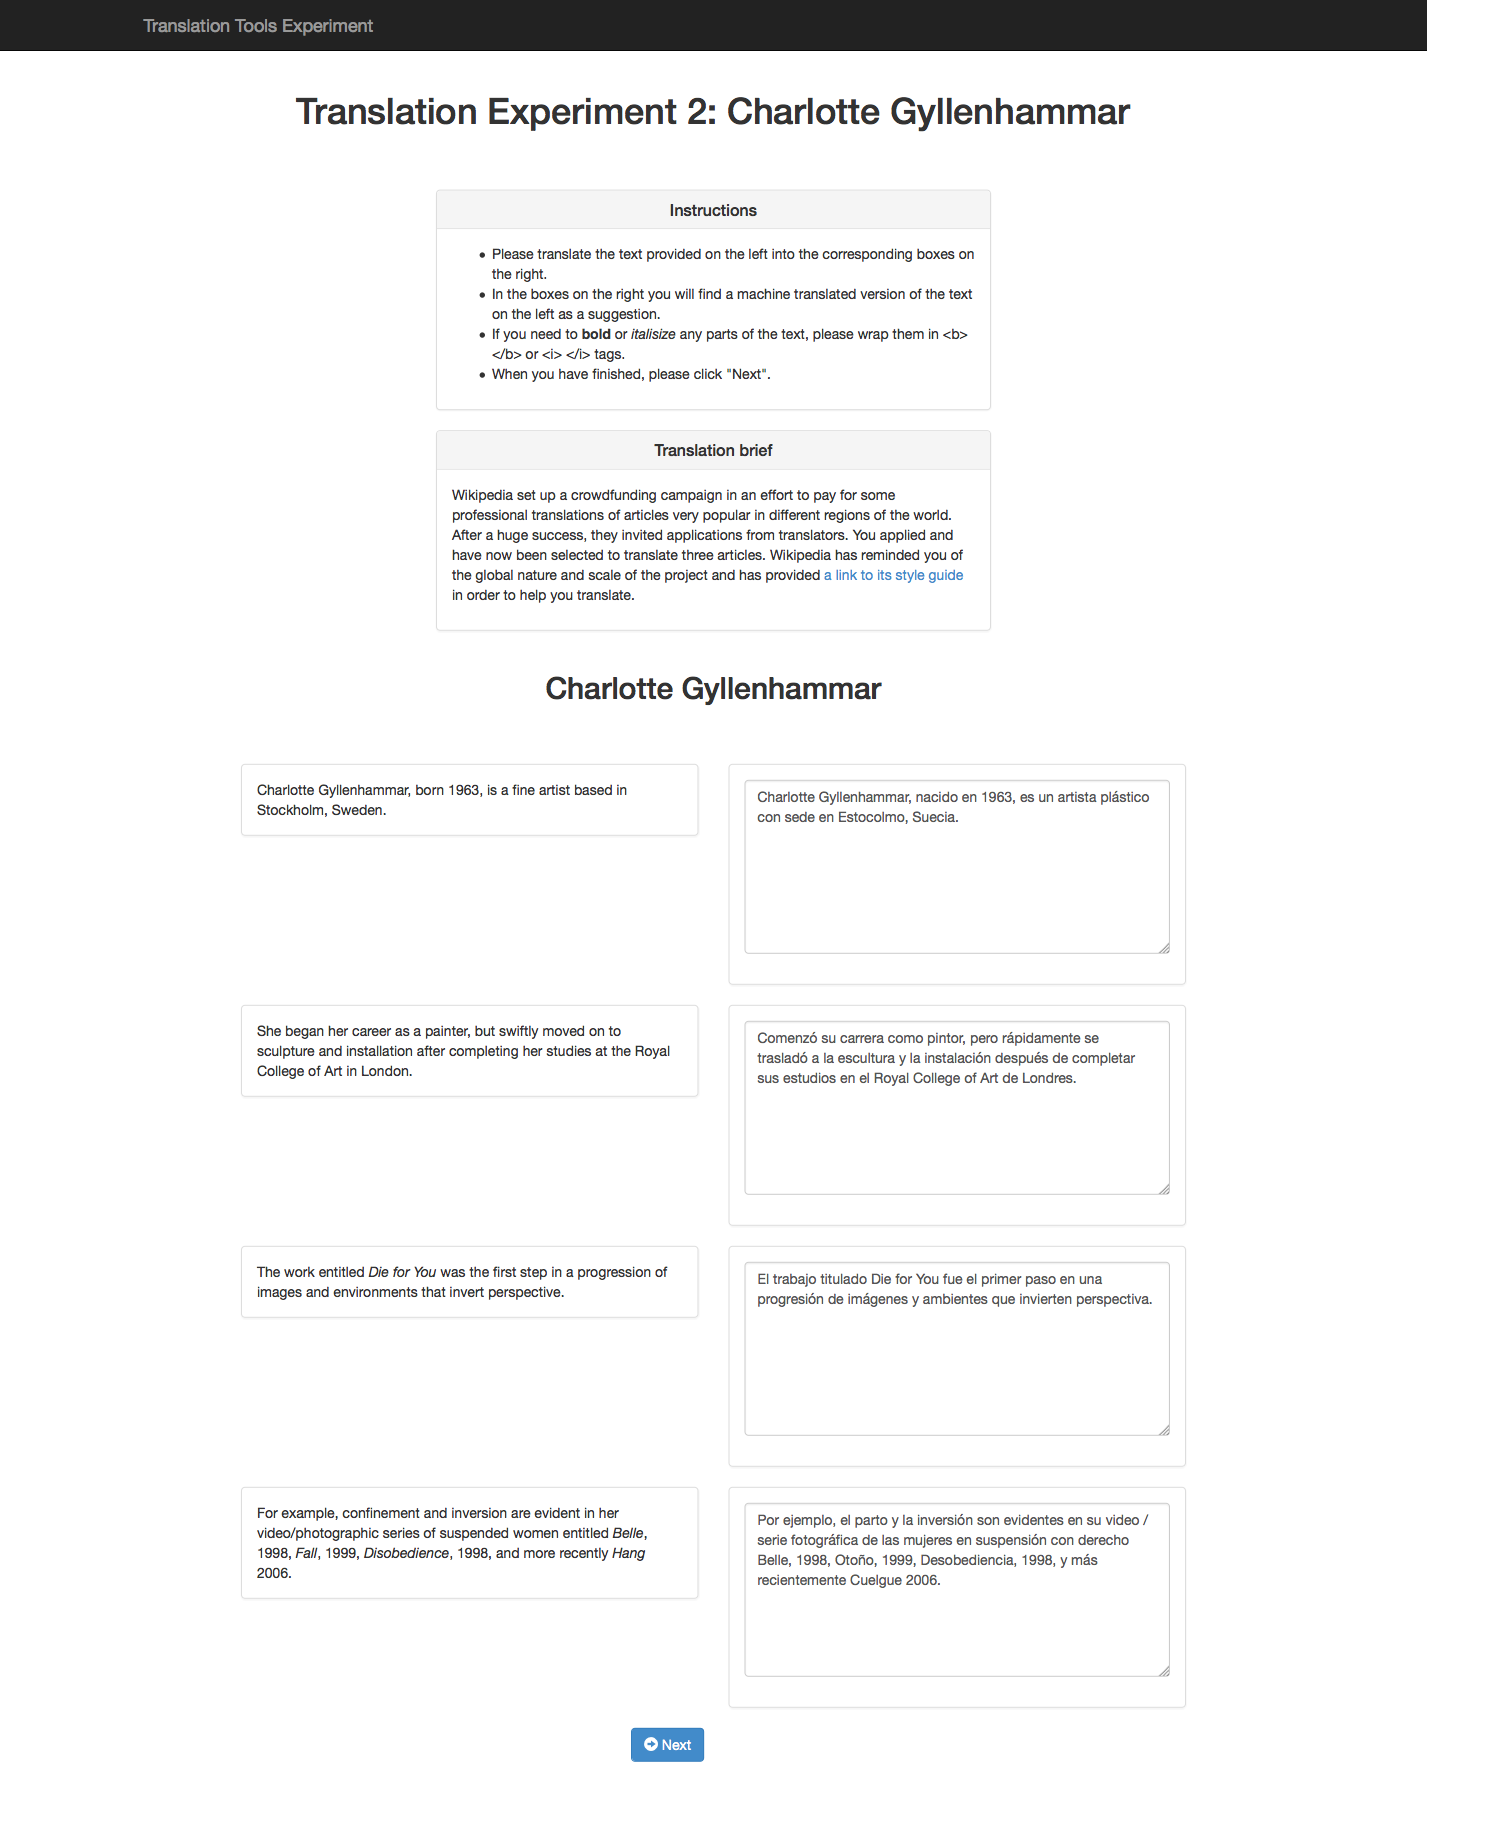
\includegraphics[width=\textwidth]{img/web/web_5.png}
\caption{Website (Page 5). Participants translate in the \ac{PE} setup.}
\label{fig:web_pe}
\end{figure}

\begin{figure}[h]
\myfloatalign
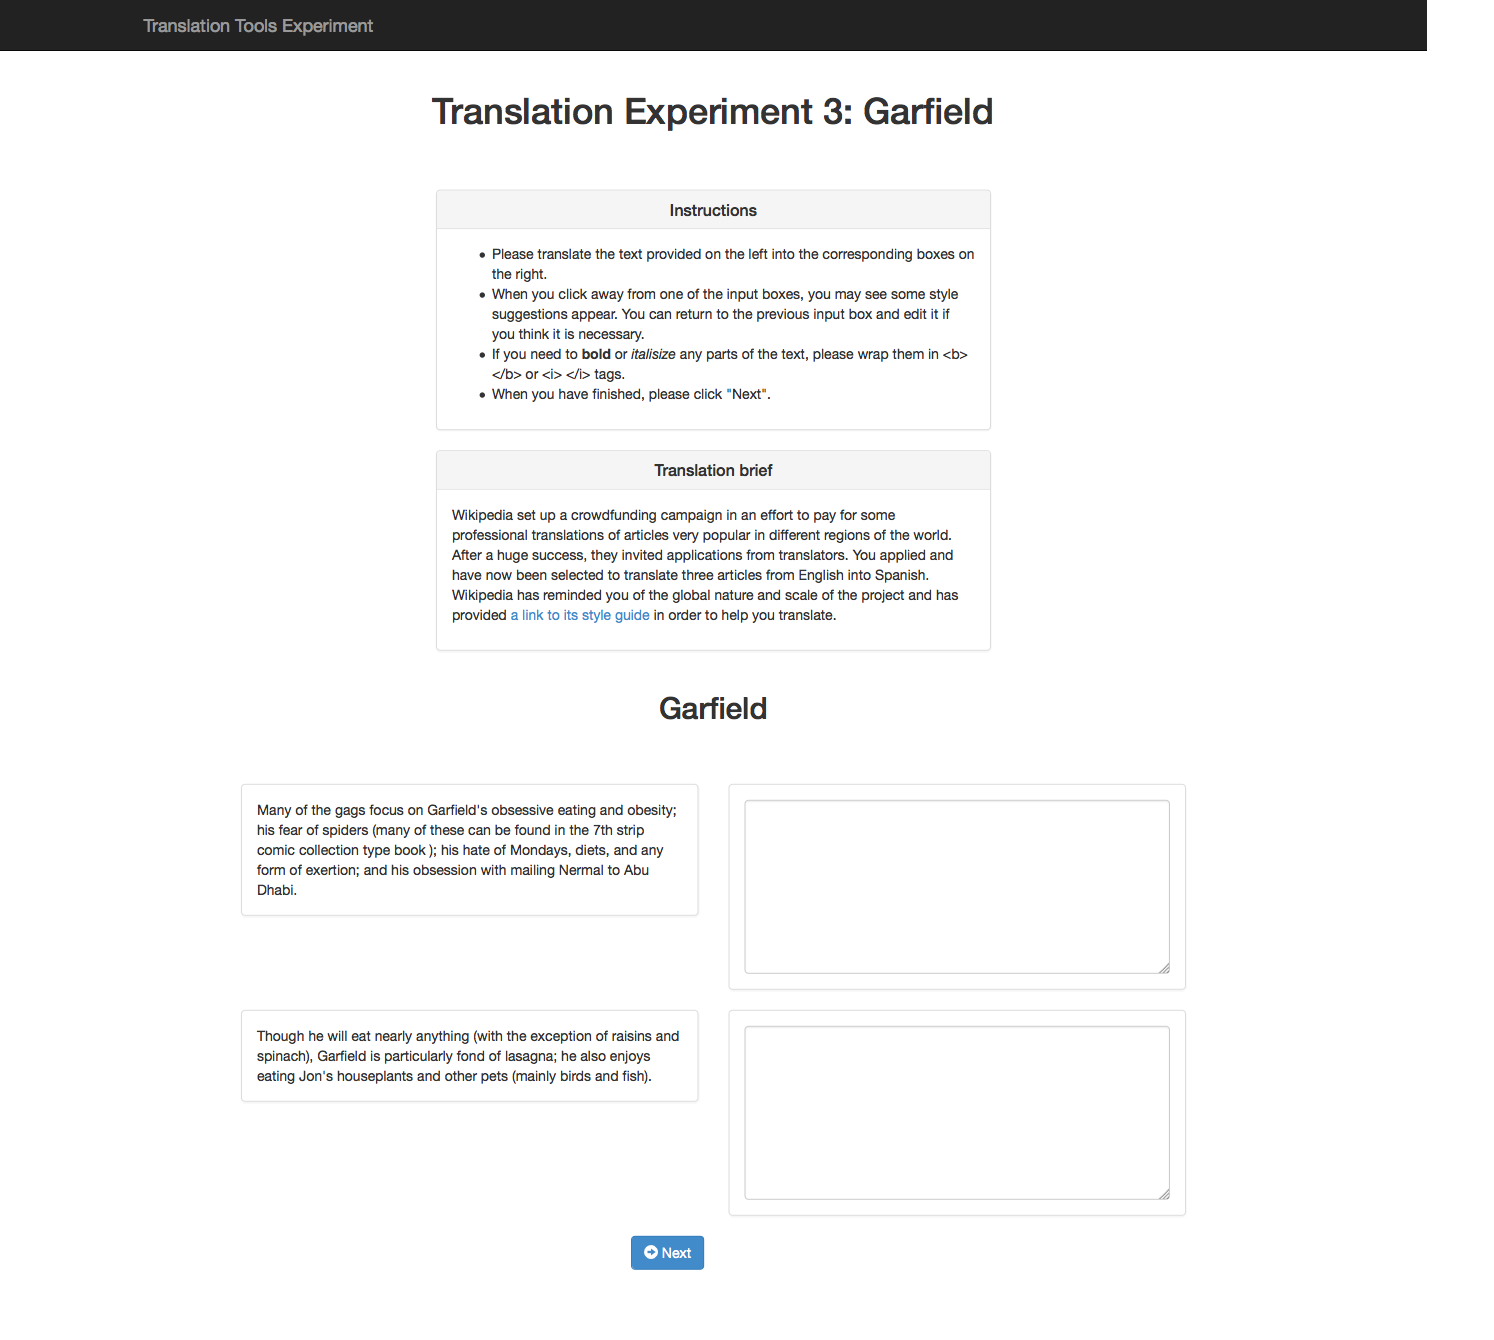
\includegraphics[width=\textwidth]{img/web/web_6.png}
\caption{Website (Page 6). Participants translate in the style setup.}
\label{fig:web_style}
\end{figure}

Finally, participants were asked to complete the final questionnaire (\autoref{fig:web_final}). They were provided with the \ac{ST} of the translations they had completed (and the \ac{MT} suggestion in the \ac{PE} setup) to help jog their memory. Finally, participants are thanked for their participation (\autoref{fig:web_thanks}).

\begin{figure}[h]
\myfloatalign
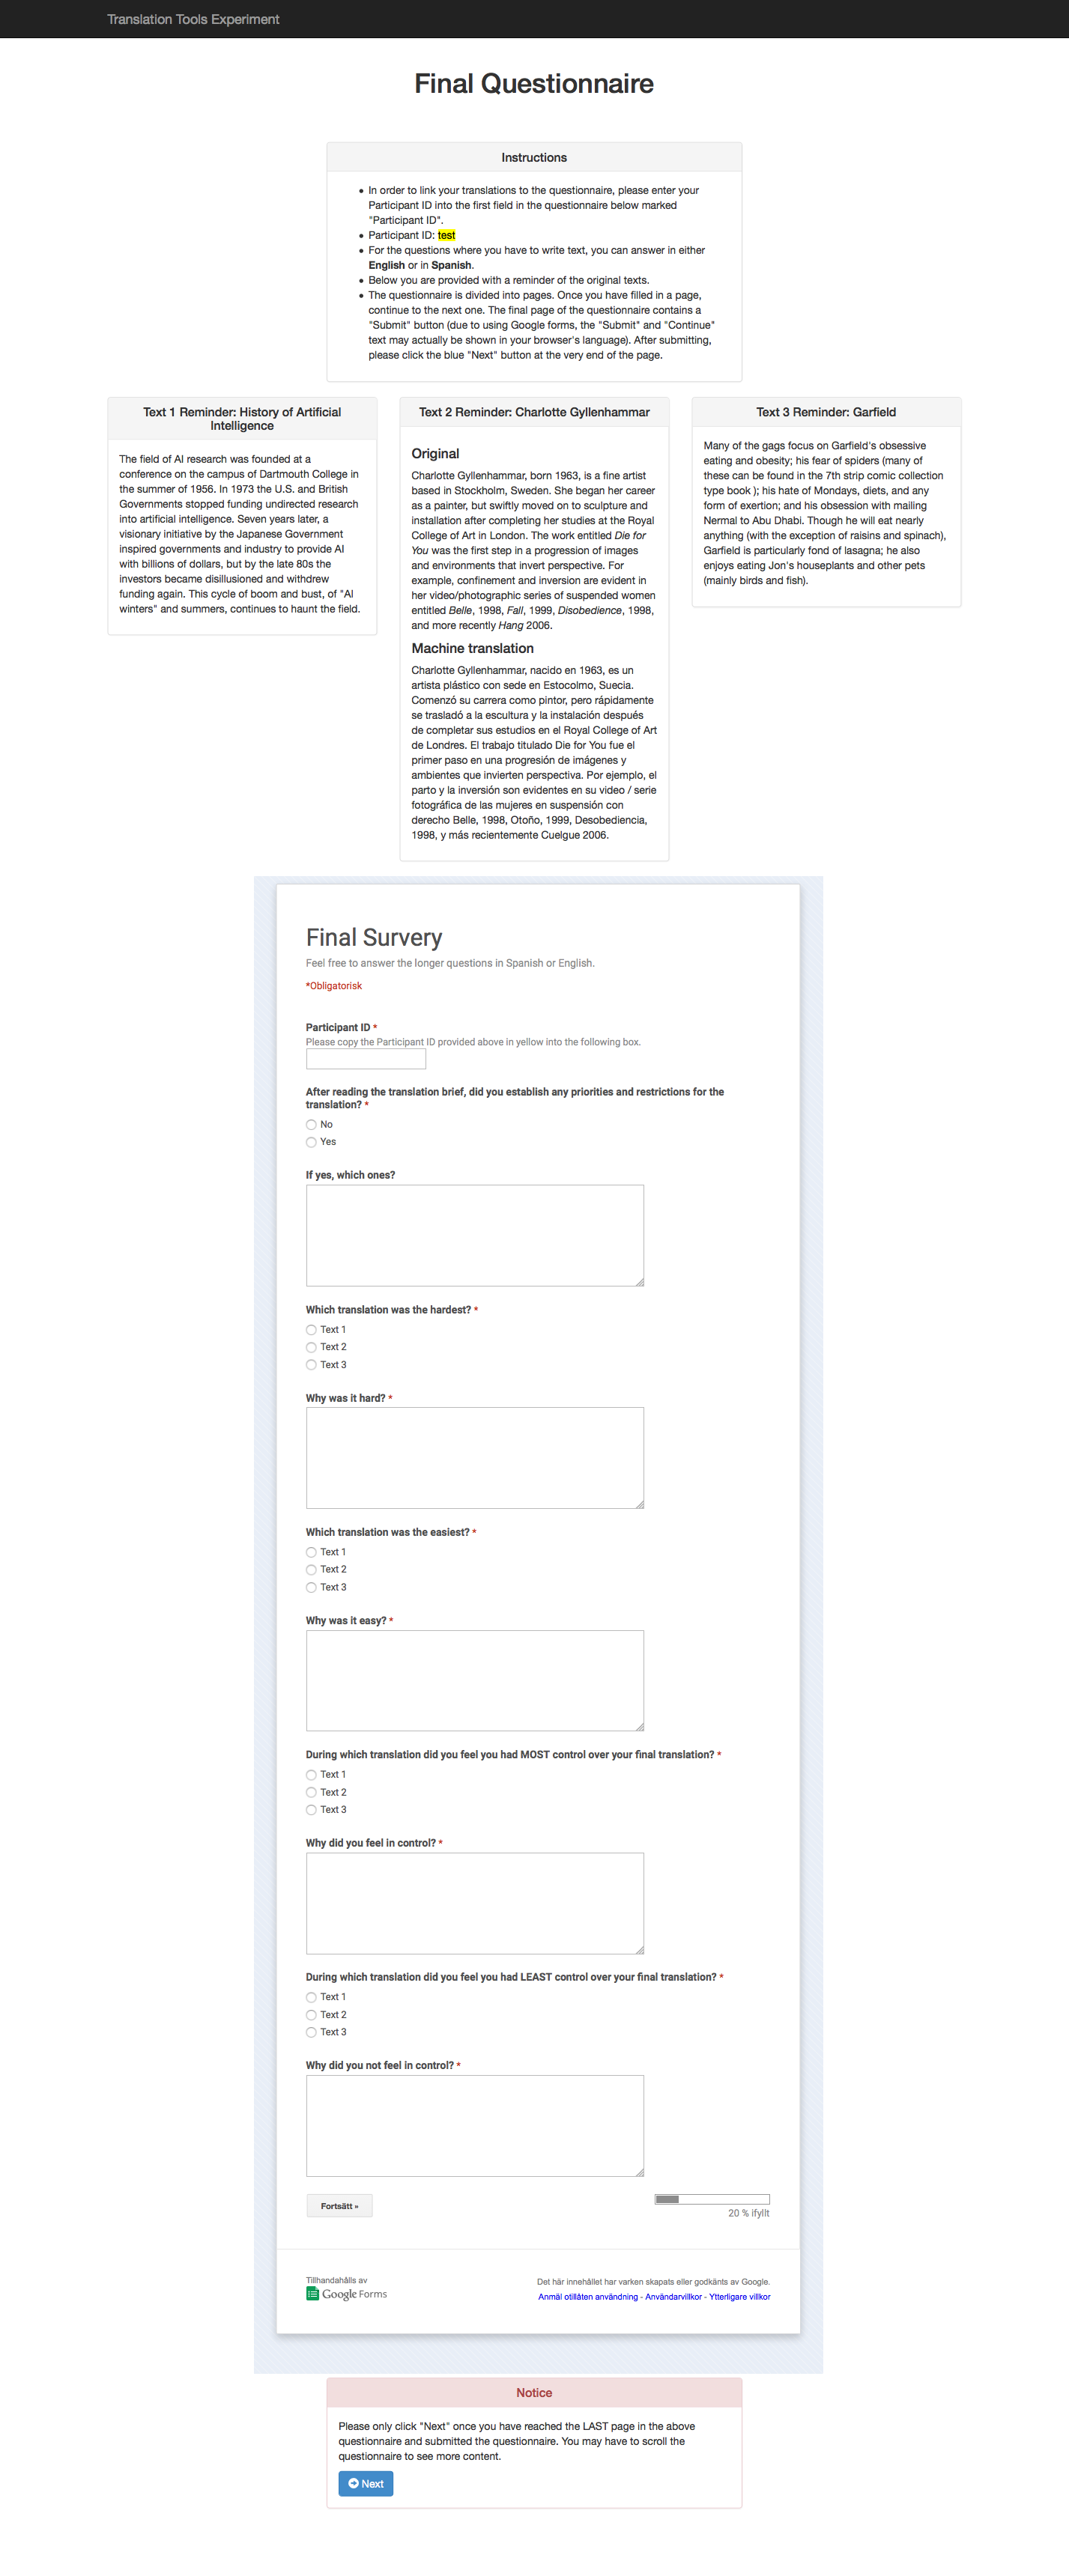
\includegraphics[height=\textheight]{img/web/web_7.png}
\caption{Website (Page 7). Participants are asked to answer the final questionnaire.}
\label{fig:web_final}
\end{figure}

\begin{figure}[h]
\myfloatalign
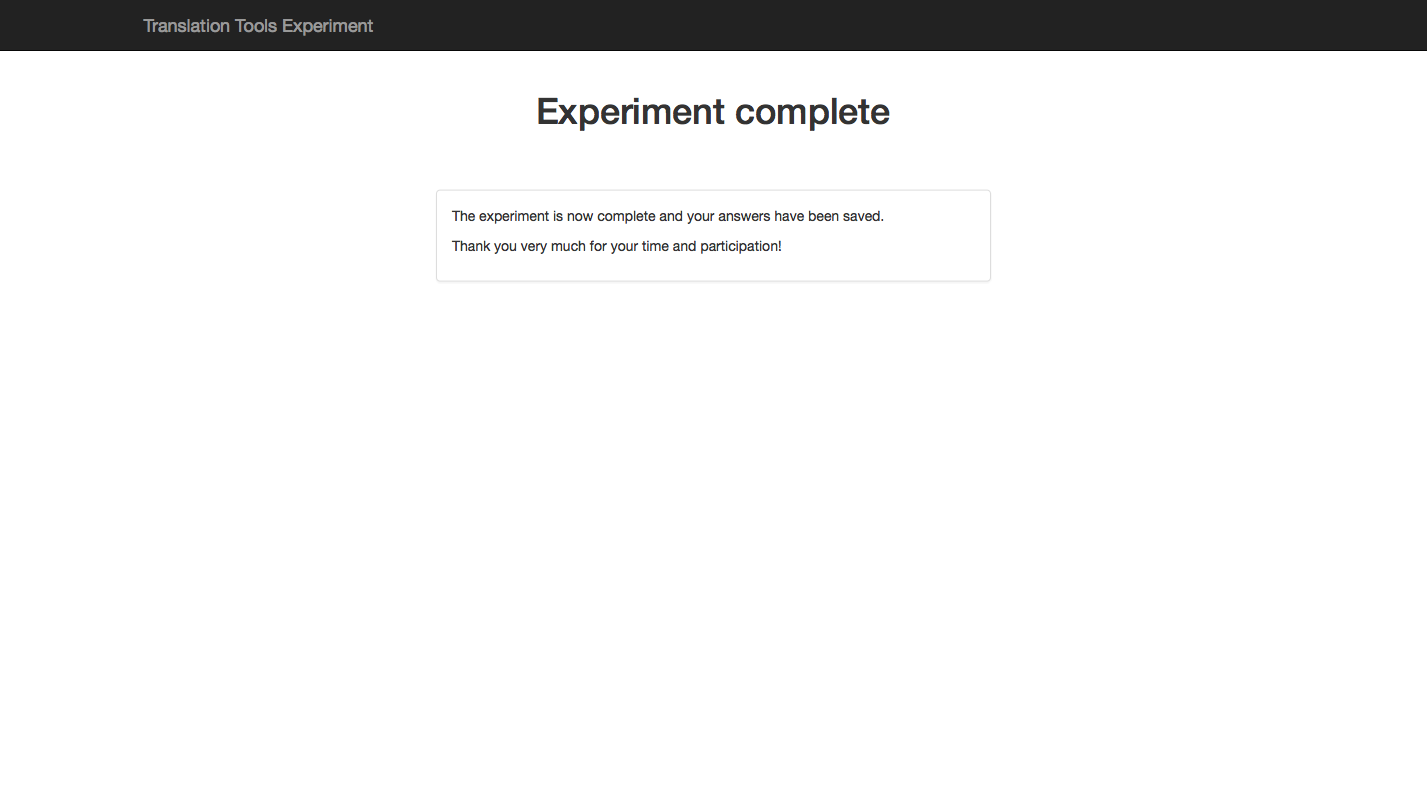
\includegraphics[width=\textwidth]{img/web/web_8.png}
\caption{Website (Page 7). Participants are thanked for their collaboration.}
\label{fig:web_thanks}
\end{figure}
